\documentclass{article}
\usepackage{main}

\title{Exercices : Nombre dérivé}
\author{Première Spécialité Mathématiques}
\date{21 Janvier 2025}

\begin{document}
\maketitle
\section{Sécantes}
Tracer sur la figure suivante une courbe représentative de fonction au crayon à papier, puis tracer une sécante entre deux points de la courbe d'abscisse $a$ et $b$.

La fonction est-elle monotone sur $[a;b]$ ?

Si ce n'est pas le cas, tracer une autre sécante en conservant l'abscisse $a$ (et en changeant l'abscisse $b$).

Existe-t-il alors une courbe n'étant pas monotone entre $a$ et $b$ ? 

Effacer votre courbe et tracer un contre-exemple possible.

Continuer cette procédure deux ou trois fois. La sécante est-elle le bon outil pour étudier la monotonie d'une fonction ?
\begin{center}
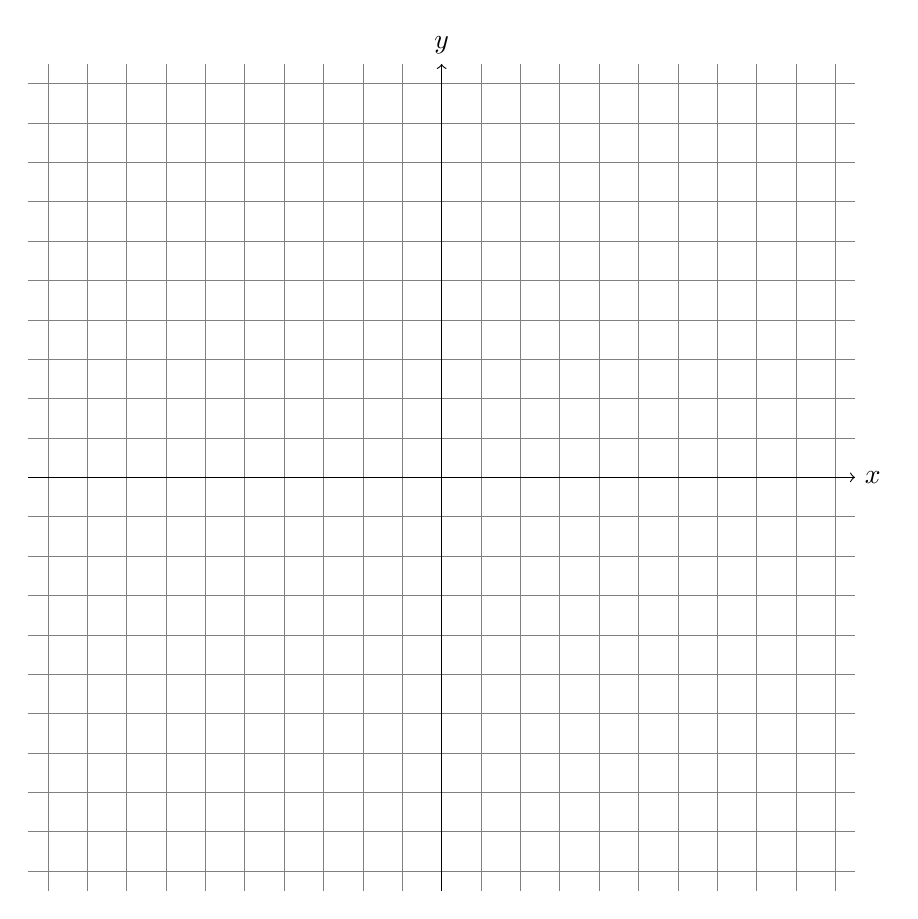
\begin{tikzpicture}
\draw[help lines] (-5.25,-5.25) grid[step=0.5] (5.25,5.25);
\draw[->] (-5.25,0) -- (5.25,0) node[right] {$x$};
\draw[->] (0,-5.25) -- (0,5.25) node[above] {$y$};
\end{tikzpicture}
\end{center}
\section{Application}
\begin{tcolorbox}
Pour chacune des fonctions $f$ suivantes, calculer le taux de variation entre la valeur $a$ fixée et $b = a+h$ en fonction de $h$. En déduire l'existence possible d'une limite en $0$.
\end{tcolorbox}
\begin{enumquestions}
\item $f(x) = 5x^2-x+7$; $a = 1$
\item $f(x) = 2x^2-3$; $a = 2$
\item $f(x) = \dfrac{3}{x^2 + 1}$; $a = -2$
\item $f(x) = (x-3)(x+1)$; $a = 3$
\item $f(x) = 2(x+1)^2+2$; $a = 3$
\end{enumquestions}
\end{document}